% Appendix A

\chapter{Propagation of calibration errors into the estimated source 
parameters}
\label{AppendixA}

In order to understand the propagation of systematic errors from calibration 
parameters to the estimated source parameters, a simple simulation is made 
as follows.

\section{DARM feedback loop modeling}

As discussed in Chapter~\ref{Chapter1}, the response function of 
interferometer system $R(f)$ can be written as 
\begin{equation}
R(f) = \frac{1+G(f)}{C(f)}
\end{equation}
where $G(f) = C(f)D(f)A(f)$ is the DARM open loop gain, $C(f)$ is the sensing 
function, $D(f)$ is the digital filters and $A(f)$ is the actuator function.
As a typical configuration, we used $G(f)$ and $A(f)$ based on the LIGO O1/O2 
configuration~\cite{LIGO-CAL,Tuyenbayev}. Fig.~\ref{fig:appa-olg} shows the 
transfer functions of open loop gain and actuators. Here we assume the 
three-stage pendulum and second and third stages contribute the control 
in the frequency range we are interested in. For the sensing function, 
in the case without Signal Recycling Cavity (SRC) detuning, $C(f)$ 
can be approximated by a single pole,
\begin{equation}
C(f)=\frac{G_c}{1+{\rm i}f/f_c},
\end{equation}

where $G_c$ is the optical gain, $f_c$ is the coupled cavity pole frequency.

In this simulation, we assume three parameters, $G_c$, $f_c$ and $A_T$ 
to be calibrated and tracked, where $A_T$ is the scale factor of 
the actuator function. Figs.~\ref{fig:appa-cal1},\ref{fig:appa-cal2} and
\ref{fig:appa-cal3} show the deformations 
of $R(f)$ due to the calibration bias on these three parameters.
These results agree with Ref~\cite{Tuyenbayev}. Since the assumed 
transfer functions are not exactly the same as Ref~\cite{Tuyenbayev} 
there are minor differences.

\begin{figure}
\begin{center}
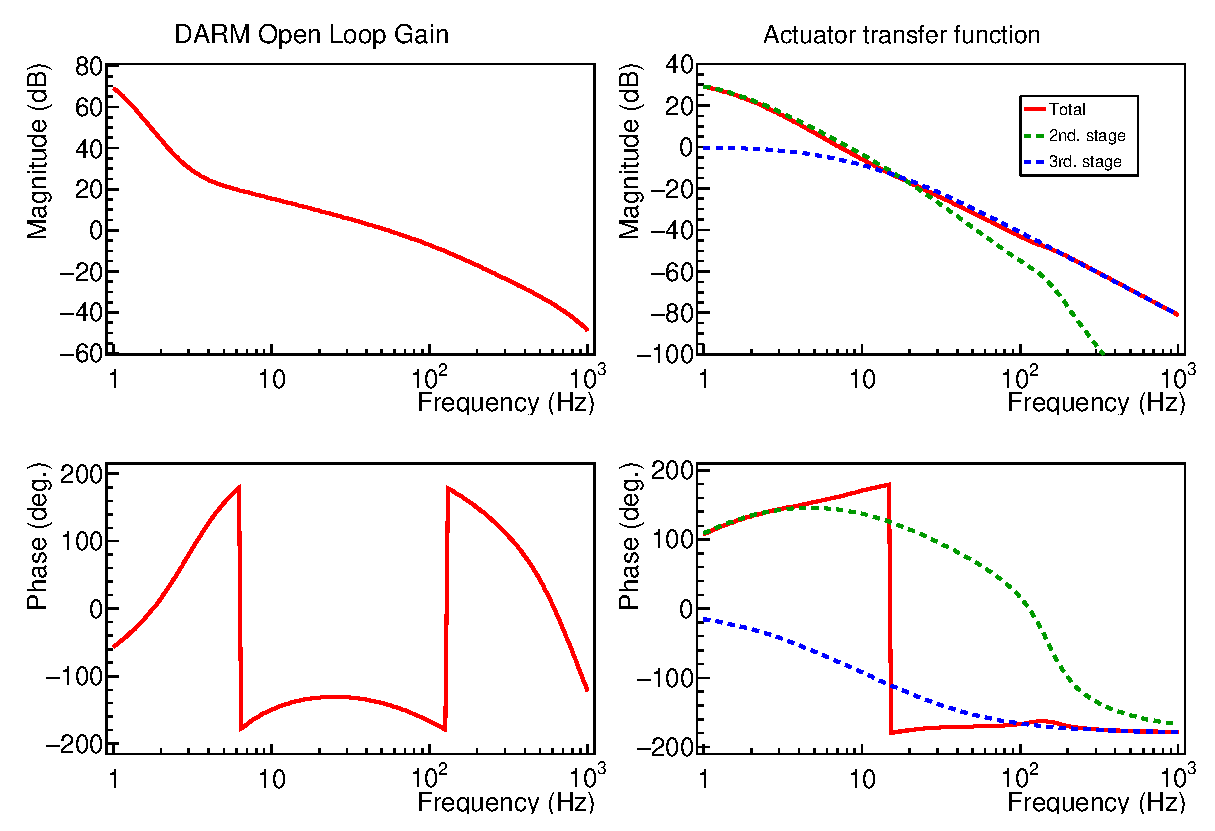
\includegraphics[width=\linewidth]{Figures/appa-olg.eps}
\caption{Transfer functions of DARM open loop gain and actuators assumed in 
this simulation.}
\label{fig:appa-olg} 
\end{center}
\end{figure}

\begin{figure}
\begin{center}
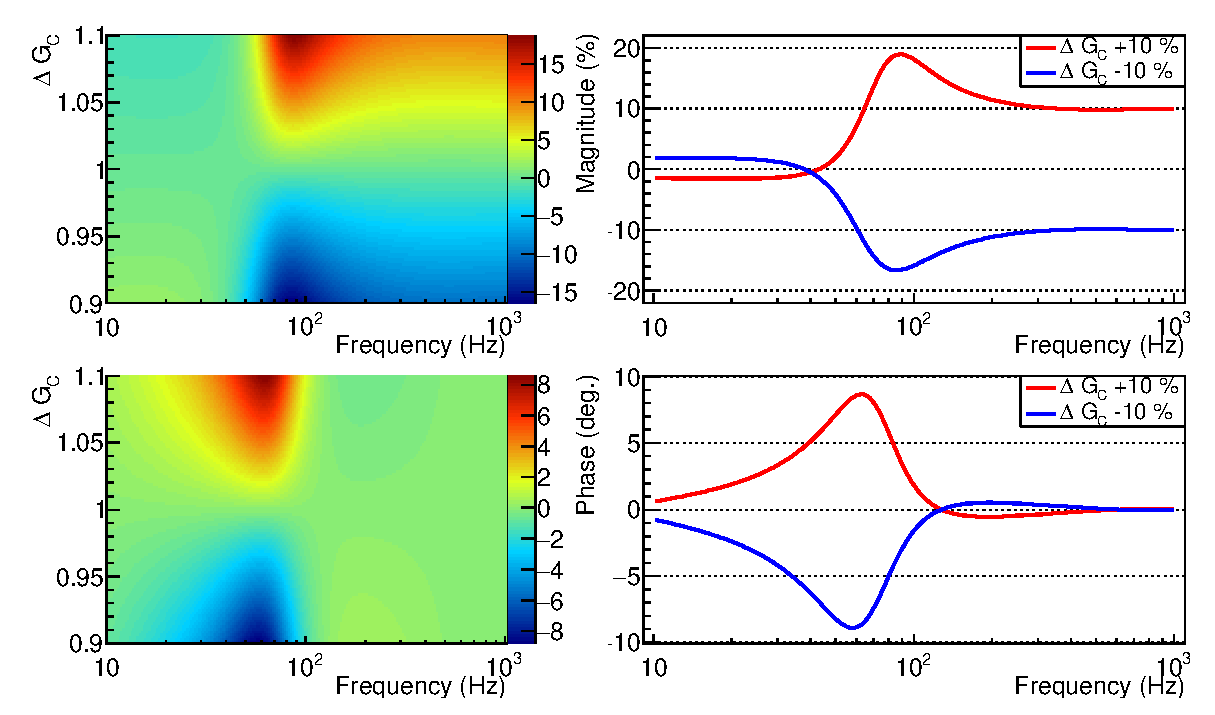
\includegraphics[width=\linewidth]{Figures/appa-cal1.eps}
%\includegraphics[width=\linewidth]{Figures/appa-cal1k.eps}
\caption{Deformation of $R(f)$ due to the relative calibration bias on $G_C$.}
\label{fig:appa-cal1} 
\end{center}
\end{figure}

\begin{figure}
\begin{center}
\includegraphics[width=\linewidth]{Figures/appa-cal2.eps}
\caption{Deformation of $R(f)$ due to the relative calibration bias on $f_C$.}
\label{fig:appa-cal2} 
\end{center}
\end{figure}

\begin{figure}
\begin{center}
\includegraphics[width=\linewidth]{Figures/appa-cal3.eps}
%\includegraphics[width=\linewidth]{Figures/appa-cal3k.eps}
\caption{Deformation of $R(f)$ due to the calibration bias on $A_T$.}
\label{fig:appa-cal3} 
\end{center}
\end{figure}

\newpage
\section{Waveform modeling}
As a simple example, we assume the GW signal in the frequency domain from 
the compact binary coalescence by using the second order post-Newtonian (2-pN) 
formalism and ignoring any effects due to the spins with five free parameters, 
a total system mass, $M=m_1+m_2$,
a symmetric mass ratio $\eta=m_1 m_2/M^2$, the source distance, $D$, 
a coalescence time $t_c$, and a coalescence phase $\phi$,
\begin{equation}
h(f) = \frac{1}{2\pi^{2/3}c^{3/2}}\frac{(GM)^{5/6}}{D}\left(\frac{5\eta}{6}\right)^{1/2}f^{-7/6} e^{i(2\pi ft_c+\phi+\Psi(f))},
\end{equation}
where 
\begin{equation}
\Psi(f)=\sum_{i=1}^4 a_i \xi_i(f),
\end{equation}
\begin{equation}
a_1=\frac{3}{128\eta}q^{-5/3},
\end{equation}
\begin{equation}
a_2=\frac{1}{384\eta}\left(\frac{3\:715}{84}+55\eta\right)q^{-1},
\end{equation}
\begin{equation}
a_3=-\frac{1}{128\eta}48\pi q^{-2/3},
\end{equation}
\begin{equation}
a_4=\frac{3}{128\eta}\left(\frac{15\:293\:365}{508\:032}+
\frac{27\:145}{504}\eta+\frac{3\:085}{72}\eta^2\right)q^{-1/3},
\end{equation}
$\xi_1(f)=f^{-5/3}$, $\xi_2(f)=f^{-1}$, $\xi_3(f)=f^{-2/3}$, 
$\xi_4(f)=f^{-1/3}$, and $q=\pi GMc^{-3}$~\cite{Tanaka-Tagoshi}.

The parameters estimation is done with the maximum likelihood method, 
\begin{equation}
{\rm ln}L = -\frac{1}{2}\int_{f_{min}}^{f_{max}}df\frac{|d(f)-h(f)|^{2}}{S(f)},
\end{equation}
where $f_{min}$ and $f_{max}$ are the filtered frequency range, 
$d(f)$ and $h(f)$ are observed and estimated wave forms, and 
$S(f)$ is the power spectrum density of the detector noise.

In this analysis we assume the source parameters similar to GW150914 
and fittin between 30 and 300~Hz.
Fig.~\ref{fig:appa-cmp} shows the comparisons of relative deformed and fitted 
wave forms with respect to the true one. Finaly, we estimated the bias on 
the five source parameters. Left part of Fig.~\ref{fig:appa-sim} shows 
the systematic bias on the five source parameters, while rigt part of 
Fig.~\ref{fig:appa-sim} shows the extreme case where the source distance is 
200~Mpc away and the signal-to-noise ratio is high enough.

\begin{figure}
\begin{center}
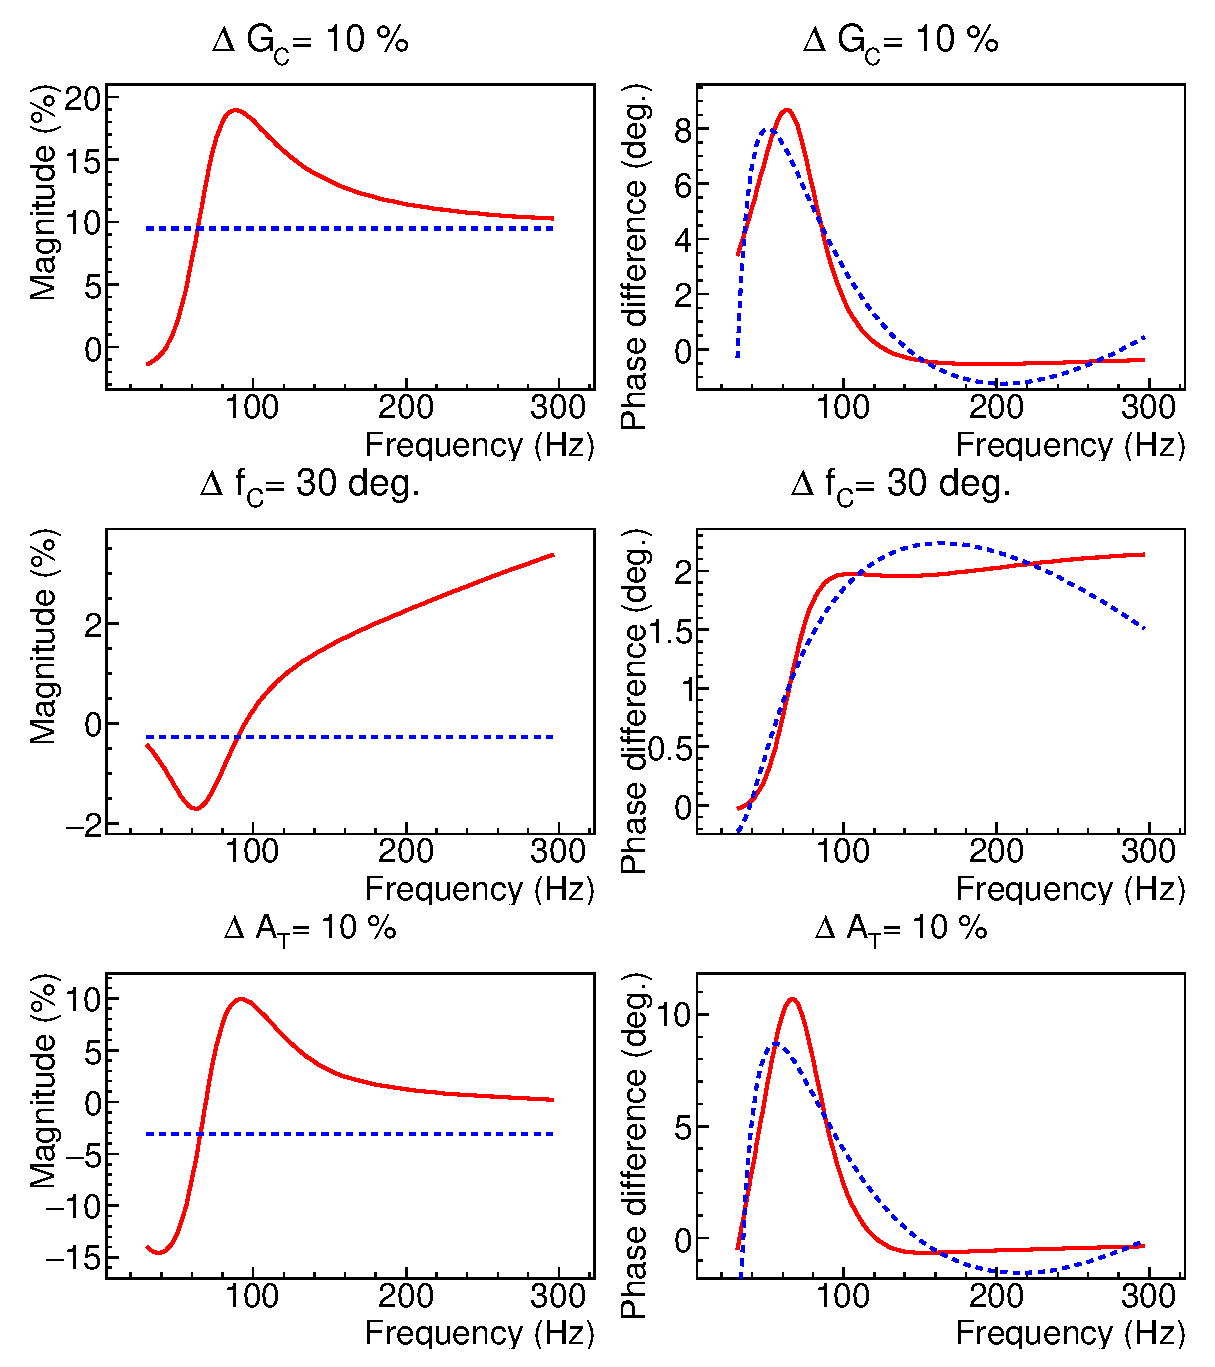
\includegraphics[width=\linewidth]{Figures/appa-cmp.eps}
\caption{Comparisons of relative deformed (red solid lines) and fitted 
(blue dashed lines) wave forms with respect to the true one, 
in the three cases where $G_C$, $f_C$ and $A_T$ are biased by 
$\pm 10\%$, $\pm 30$ deg., and $\pm 10\%$, respectively.}
\label{fig:appa-cmp} 
\end{center}
\end{figure}

\begin{figure}
\begin{center}
\includegraphics[width=0.49\linewidth]{Figures/appa-sim1.eps}
\includegraphics[width=0.49\linewidth]{Figures/appa-sim2.eps}
%\includegraphics[width=0.49\linewidth]{Figures/appa-sim1k.eps}
%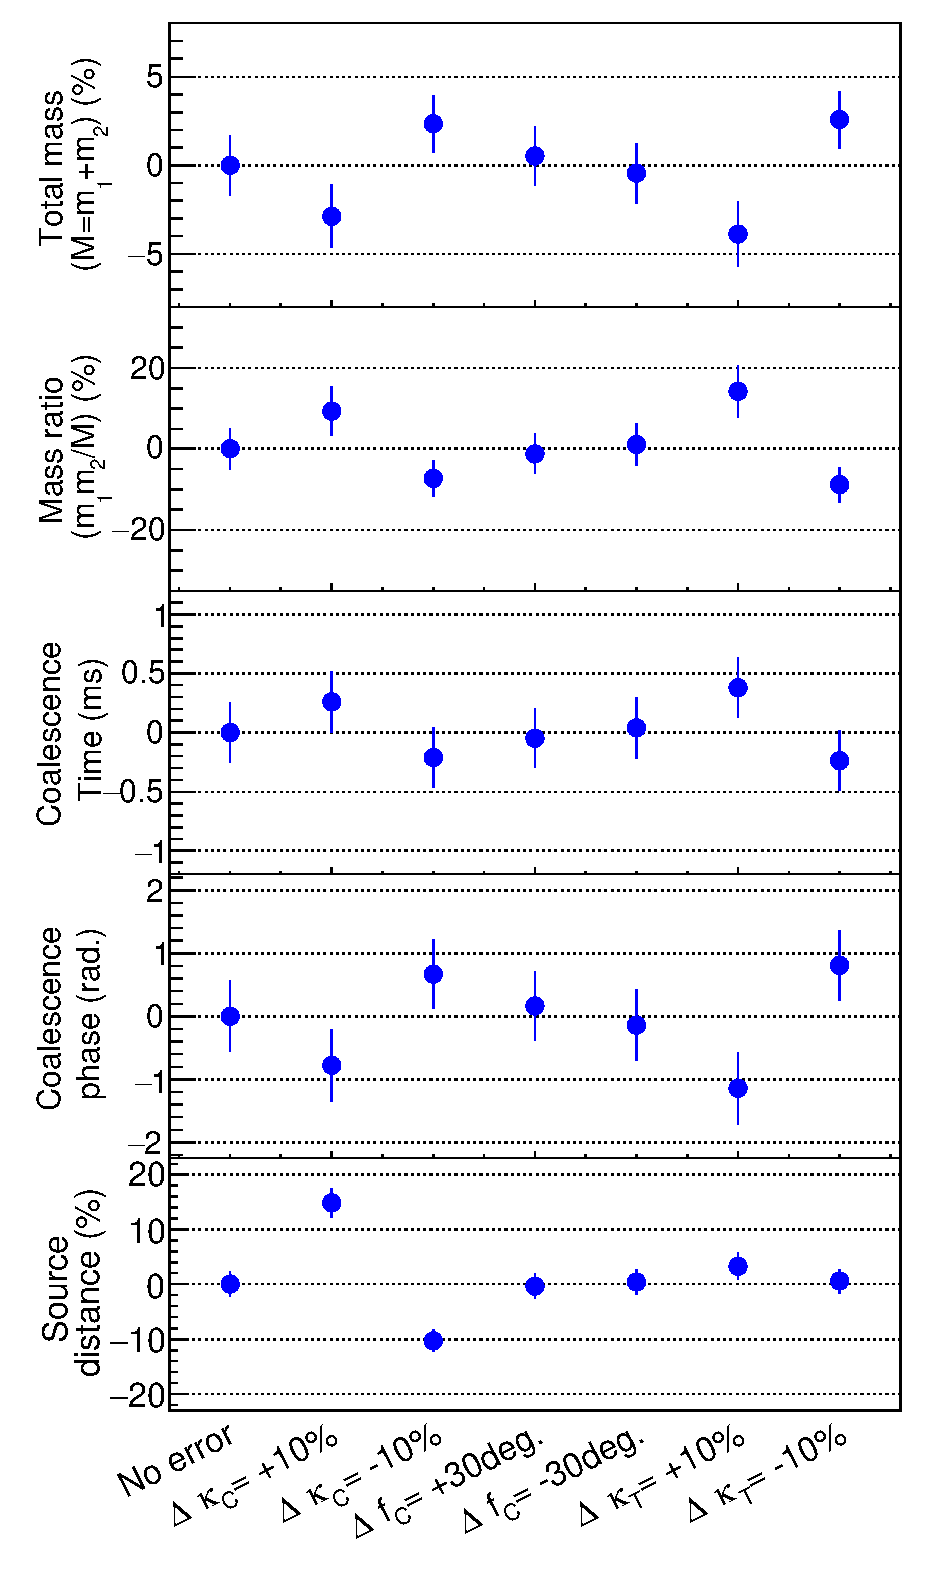
\includegraphics[width=0.49\linewidth]{Figures/appa-sim2k.eps}
\caption{The systematic bias on the five source parameters as a 
function of variations of calibration parameters assuming the 
signal similar to GW150914 (left), and the extreme case where 
the GW150914 source is 200~Mpc away (right).}
\label{fig:appa-sim} 
\end{center}
\end{figure}
